\documentclass[10pt,a4paper]{article}
\usepackage[a4paper,margin=1.9cm]{geometry}
\usepackage[T1]{fontenc}
\usepackage{lmodern,microtype,amsmath,booktabs,graphicx,xcolor,caption}
\usepackage[hidelinks]{hyperref}
\usepackage{titlesec}
\titlespacing*{\section}{0pt}{1.0ex}{0.4ex}
\captionsetup{font=small,labelfont=bf,skip=3pt}
\setlength{\parskip}{0.3ex}
\setlength{\textfloatsep}{8pt}
\setlength{\emergencystretch}{1.5em}
\newcommand{\code}[1]{\texttt{#1}}
\newcommand{\todo}[1]{\par\noindent\colorbox{yellow!40}{\parbox{\dimexpr\linewidth-2\fboxsep}{\small\textbf{TODO:} #1}}\par}

\title{\vspace{-1.4cm}CITS3402/5507 Assignment 2: a distributed birthday attack with MPI and OpenMP}
\author{Shaoming Wu (24914408)}
\date{October 2026}

\begin{document}
\maketitle

\section{Algorithm and workload decomposition}
A \emph{trial} hashes file A or B with one 64-bit nonce, written as 16 hex digits at byte 16. With
$n$ trials per file about $n^2/2^{48}$ cross-file collisions are expected. The $K$-th collision
therefore needs $2^{25}\Gamma(K{+}\tfrac12)/\Gamma(K)\approx2^{25}\sqrt K$ trials ($3.0\times10^7$
for $K{=}1$), and every trial must be stored until it is matched.

Process $r$ uses nonces $s\,2^{56}+r\,2^{40}+c$, so trials are never repeated, need no coordination,
and every process does equal work. Units of eight nonces alternate between A and B, keeping both
populations equal.

The FNV state of the 16-byte prefix is cached; a trial then hashes the nonce and the remaining
64--920\,KiB. One FNV chain is limited by multiply latency, so the kernel advances eight nonces over
each byte together, giving 7.3$\times$ the single-chain throughput. We also derived an exact shortcut. Because $h\oplus c=h+c-2(h\wedge c)$, and
the low byte of an FNV state depends only on the previous low byte, the suffix map is
$S(h)=P^{n}h+C[h \bmod 256] \pmod{2^{64}}$, so a trial costs only 16 steps (\code{--fast}). As it
removes the intended workload, we use it only to expose communication limits.

\section{Distributed collision detection}
Process $h \bmod p$ owns hash $h$ and stores only its own hashes in an open-addressing table. The
table is indexed by a multiplicative hash, so slot positions do not depend on $h \bmod p$. A record
that meets a stored record from the other file is a collision, and the slot is then marked. Each hash
therefore has one owner and is reported once, so collisions are globally distinct with no extra
messages. \code{toy\_hash} ends in a 64-bit finaliser, so ownership is uniform. Owners receive
$N/p\pm\sqrt{N/p}$ records, which balances work and memory to within 0.1\% at $N/p{=}10^6$.

\section{Communication, batching and termination}
Each process buffers $B$ 16-byte records per destination; records it owns are inserted directly. Full
buffers are sent with \code{MPI\_Issend}, at most two in flight per destination. Synchronous sends
make this credit-based flow control; with eager \code{MPI\_Isend}, producers flooded slower owners. Owners receive with \code{MPI\_Improbe}/\code{MPI\_Mrecv}, at most
$p$ messages per poll, and every waiting loop keeps receiving, which rules out deadlock. The master
also polls MPI between its own work units. Without asynchronous progress, rendezvous transfers
otherwise waited a whole iteration, which cost 25\% of throughput at $B{=}1024$. A larger $B$ means
fewer messages but later detection: a buffer fills at rate $r/p$, delaying candidates by up to
$Bp/r$, which \code{--flush-ms} (default 100\,ms) caps.

To terminate, each process keeps one \code{MPI\_Iallreduce} of its collision count in flight. All
processes see the same totals, so they stop at the same reduction once the total reaches $K$, with no
coordinator. They then exchange per-peer message counts (\code{MPI\_Ialltoall}) and drain all
in-flight batches. Rank~0 gathers the collisions (\code{MPI\_Gatherv}) and verifies each of the first
$K$ on its own, by patching the original files and recomputing \code{toy\_hash}, before writing.
Benchmark mode runs exactly $N$ trials through the same pipeline and never stops early.

\section{Hybrid MPI+OpenMP}
Each process runs one parallel region. While the team hashes chunk $i$ into one of two record
buffers (\code{schedule(dynamic,1)}), the master routes chunk $i{-}1$, receives and inserts batches,
and tests for termination; then it joins the hashing. Lane states are private and the kernel tables
are shared read-only. Each unit writes a disjoint slice of the shared record buffer, so no locks are
needed. MPI buffers, requests and the table slice belong to the master, and loop control changes only
between barriers. Only the master calls MPI, so we request and check \code{MPI\_THREAD\_FUNNELED};
\code{MULTIPLE} would add locking that we do not need.

\begin{table}[t]
\centering\small
\caption{Per pair: single-core kernel throughput (trials/s), and the 8-core hybrid ($2\times4$) run
that produced the submitted files: time $t_1$ and the trials it used.}
\label{tab:pairs}
\begin{tabular}{lrrrrr}
\toprule
 & & \multicolumn{4}{c}{Apple M4 (dev.)}\\
pair & KiB & full/s & fast/s & $t_{1}$ (s) & trials (M)\\
\midrule
1\_alpha & 65 & 113.4\,k & 46.2\,M & 82.9 & 37.0\\
2\_beta & 130 & 57.0\,k & 46.1\,M & 87.5 & 18.5\\
3\_gamma & 230 & 32.2\,k & 46.3\,M & 128.8 & 15.1\\
4\_delta & 350 & 21.2\,k & 45.6\,M & 273.8 & 21.4\\
5\_epsilon & 500 & 14.7\,k & 45.1\,M & 140.8 & 7.8\\
6\_zeta & 920 & 8.0\,k & 45.4\,M & 480.3 & 14.9\\
\bottomrule
\end{tabular}

\end{table}

\begin{figure}[t]
\centering
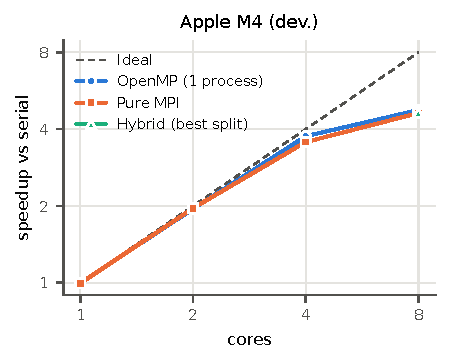
\includegraphics[width=0.49\linewidth]{figures/scaling.pdf}\hfill
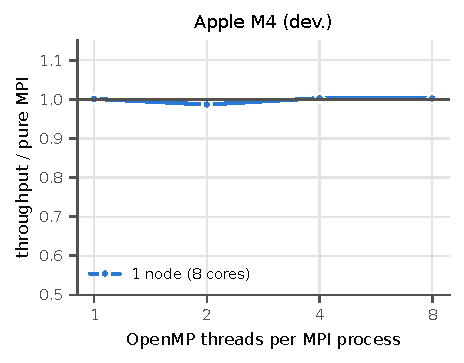
\includegraphics[width=0.49\linewidth]{figures/hybrid.pdf}
\caption{Fixed-work scaling (gamma, best of three runs). Left: speedup. Right: hybrid throughput
relative to pure MPI.}
\label{fig:scaling}
\end{figure}

\begin{table}[t]
\centering\small
\caption{Fixed-work results for whole nodes (best split).}
\label{tab:scaling}
\begin{tabular}{lrrrrrr}
\toprule
program & nodes & ranks$\times$thr. & cores & $X$ & $S$ & $E$\\
\midrule\multicolumn{7}{l}{\textit{Apple M4 (dev.)}, 8 cores per node}\\
serial & 1 & 1$\times$1 & 1 & 32.4\,k & 1.0 & 100\%\\
OpenMP & 1 & 1$\times$8 & 8 & 153.6\,k & 4.7 & 59\%\\
MPI & 1 & 8$\times$1 & 8 & 149.6\,k & 4.6 & 58\%\\
hybrid & 1 & 2$\times$4 & 8 & 149.8\,k & 4.6 & 58\%\\
\bottomrule
\end{tabular}

\end{table}

\begin{figure}[t]
\centering
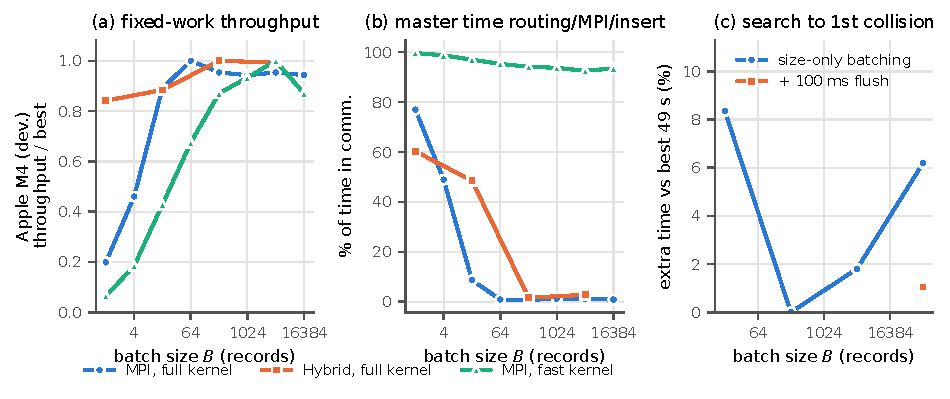
\includegraphics[width=\linewidth]{figures/batch.pdf}
\caption{Batch size $B$ (8 processes, alpha): (a) throughput; (b) master time spent communicating,
which the hybrid overlaps with hashing; (c) time to the first collision (fixed seed), relative to the fastest $B$.}
\label{fig:batch}
\end{figure}

\begin{figure}[t]
\centering
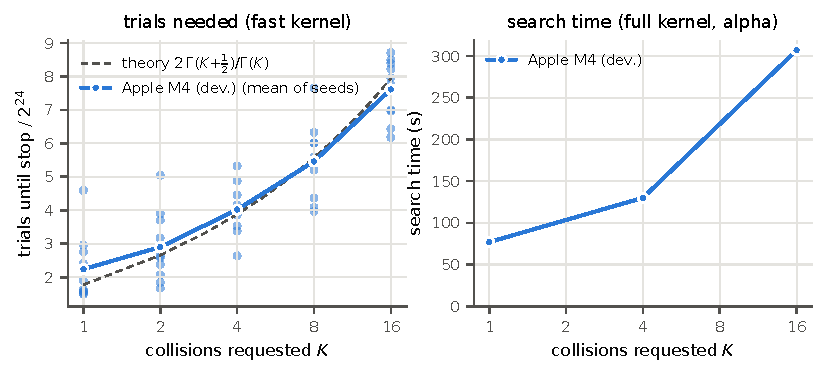
\includegraphics[width=0.9\linewidth]{figures/kcoll.pdf}
\caption{$K$ distinct collisions (alpha, 8 cores). Left: trials for each seed and their mean, against
theory. Right: full-kernel search time.}
\label{fig:k}
\end{figure}

\section{Performance}
\textbf{Method.} Development runs used an Apple M4 (4 performance and 6 efficiency cores,
MPICH~4.3) with 8 processes. We report throughput $X$ (trials/s), speedup $S=X/X_{\mathrm{serial}}$
and efficiency $E=S/\mathrm{cores}$.
%TC:ignore
\todo{Kaya and Setonix: run \code{sbatch --nodes=\{1,2,4\} slurm/setonix.slurm} and
\code{slurm/kaya.slurm}, copy \code{results/*.jsonl} back, run \code{scripts/analyse.py} (the
figures and tables gain panels and rows automatically), and replace this box with 3--4 sentences:
multi-node $S$/$E$ of MPI versus hybrid (Table~\ref{tab:scaling}), the best ranks$\times$threads
split (Figure~\ref{fig:scaling}), $B$ at 512 processes (Figure~\ref{fig:batch}), and Kaya versus
Setonix per-core throughput.}
%TC:endignore

\textbf{Kernel and time to solution.} Full-kernel throughput falls with file size, from 113\,k to
8.0\,k trials/s per core (Table~\ref{tab:pairs}). Collisions took 83--480\,s on 8 cores, depending
also on the random number of trials (7.8--37\,M). The fast kernel sustains about 46\,M trials/s on
every pair.

\textbf{Fixed-work scaling.} On the four performance cores, all programs reach $S=3.6$--$3.8$
($E\ge89\%$), and communication takes under 1\% of the time (Figure~\ref{fig:scaling},
Table~\ref{tab:scaling}). Beyond four cores the curve flattens to $S\approx4.7$ at eight, because
the extra cores are efficiency cores, about a third as fast. Every ranks$\times$threads split is
within 2\% of pure MPI, since the master's communication overlaps with hashing.

\textbf{Batch size.} Small batches are message-bound (Figure~\ref{fig:batch}). At $B{=}1$, 1.8\,M
messages, and only $2B$ records per owner poll under the credit limit, cut throughput to 20\% of peak
with the full kernel and 6\% with the fast kernel. From $B\approx64$ the full kernel is
compute-bound, while the communication-bound fast kernel keeps improving until $B{=}4096$ (72\,M
trials/s). Hybrid $2\times4$ keeps 84\% at $B{=}1$, because it has a quarter of the destinations and
hides messages behind hashing. In search mode, $B{=}65536$ added 5\% extra trials; the 100\,ms flush
removed them.

\textbf{Multiple collisions.} Over ten seeds, mean trials are within 5\% of
$2^{25}\Gamma(K{+}\frac12)/\Gamma(K)$ for $K\ge2$ (Figure~\ref{fig:k}). $K{=}1$ is within its
$\pm52\%$ spread. $K{=}16$ therefore costs about 4.5$\times$ the work of $K{=}1$, not 16$\times$,
because every stored record can pair with every later one; with the full kernel it took 307\,s
against 77\,s. Memory grows in the same way. The stop lagged availability by only 1--5\% of trials.

\textbf{Trade-offs and scalability.} A trial hashes 64--920\,KiB but sends only 16\,bytes, so for
$B\ge64$ the attack is compute-bound and should scale almost linearly across nodes. At scale the
limits are latency and memory. The detection delay $Bp/r$ and the buffer memory of $16pB$ bytes per
process grow with $p$ (8\,MB at $p{=}512$, $B{=}1024$), and the table needs about $0.5\sqrt K$\,GB.
Hybrid divides $p$ by the number of threads and so reduces both, which makes it our choice across
nodes.

\end{document}
